\documentclass[twoside,10pt]{report}
\newcommand{\docTitle}{Hw 11}
\usepackage{/Users/bradenhoagland/latex/math2}

%\renewcommand{\theenumi}{\alph{enumi}}

\begin{document}
%\tableofcontents

{\color{blue}Problems completed: All.}

\begin{exer}[]
	Suppose $X$ retracts onto $A$ via $r$ and $p \in A$. Prove that the inclusion $i_{*}:\pi_1(A,p)\to \pi_1(X,p)$ is injective and $r_{*}:\pi_1(X,p)\to \pi_1(A,p)$ is surjective.
\end{exer}
{\color{blue}Collaborators: Saloni.}

\textbf{$i_{*}$ is injective:} Since $r$ fixes $A$, $r\circ i=1_{A}$. Then for any path $\gamma$ in $A$,
\[
	(ri)_{*}=r_{*}(i_{*}([\gamma]))=[r\circ i \circ \gamma] = [\gamma],
\] so $r_{*}i_{*}$ is the identity on $\pi_{1}(A,p)$. Then if $i_{*}([\alpha])=i_{*}([\beta])$,
\[
	[\alpha] = r_{*}(i_{*}([\alpha]))=r_{*}(i_{*}([\beta]))=[\beta],
\] so $i_{*}$ is injective.

\textbf{$r_{*}$ is surjective:} Suppose $[\beta]\in \pi_1(A,p)$, then each element of $[\beta]$ lies entirely in $A$, so each is fixed by $r$. Then
\[
	r_{*}([i\circ \beta]) = [r\circ i \circ \beta]=[\beta],
\] so $r_{*}$ is surjective.

\newpage
\begin{exer}[]
	If $r$ only satisfies $r(A)\subset A$, must $r_*$ be surjective?
\end{exer}
{\color{blue}Collaborators: None.}

No, $r_{*}$ need not be surjective. Let $X=\mathbb{R}^2$, $A=\mathbb{R}^{2}-\left\{ (0,0) \right\}$, and $p=(1,1)$, and consider the constant (and thus continuous) function
\begin{align*}
	r:X&\to A\\
	x&\mapsto p.
\end{align*}
This is not a retraction, but it does satisfy $r(A)\subset A$. Note that for all loops $\alpha \subset X$,
\[
	r_{*}([\alpha]) = [r \circ \alpha] = [ t\mapsto p].
\] 
But the fundamental group $\pi_1(A,p)$ of $A$ at $p$ has two elements: the loops containing the origin and the loops not containing the origin (the constant map $t\mapsto p$ is in the latter equivalence class). Thus the equivalence class of loops in $A$ that contain the origin is never mapped to by $r_{*}$, so it is not surjective.

\newpage
\begin{exer}[]
Draw 4 different covering spaces of $S^1\vee S^1$ and demonstrate pictorially the associated covering map.
\end{exer}
{\color{blue}Collaborators: None.}

In the below diagram, I visualize the covering map with some example neighborhoods, where the corresponding neighborhoods have the same type of border. In the tree example, all blue lines are oriented upwards and all red lines are oriented right. Each line segment is also supposed to reprsent an open interval in $\mathbb{R}$. Each evenly covered neighborhood of $S^1\vee S^1$ is mapped to many more neighrbhoods on the tree than I've shown, but it would become a mess if I tried to mark them all.

\begin{figure}[H]
	\centering
	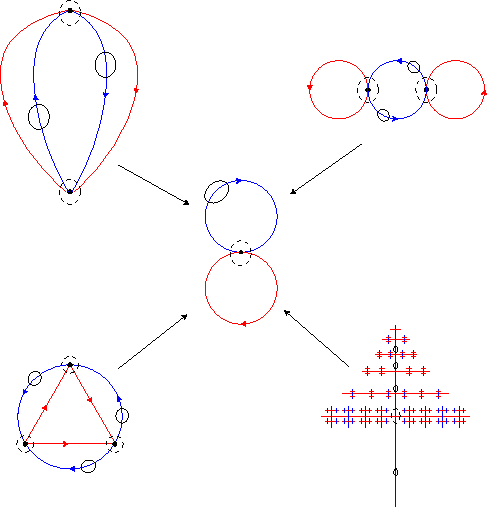
\includegraphics[scale=1.3]{fig/covers.pdf}
\end{figure}

\pagebreak
\begin{exer}[]
	Using the fact that $\pi(S^1)\cong \mathbb{Z}$, prove that $S^1\vee S^1$ is not simply connected.
\end{exer}
{\color{blue}Collaborators: None.}

Suppose $S^1\vee S^1$ is simply connected, and consider the vertex point $p$ connecting the two circles. Define a retraction $r:S^1\vee S^1\to S^1$ by retracting the bottom circle to the vertex point and fixing the top circle. Then by the first exercise, the induced homomorphism $r_{*}:\pi_1(S^1\vee S^1,p)\to \pi_1(S^1,p)$ is surjective.

Since we assumed $S^1\vee S^1$ was simply connected, this means the domain of $r_{*}$ is the trivial group. And since homomorphisms preserve identities, this means the image of $\pi_1(S^1\vee S^1,p)$ under $r_{*}$ is also just the trivial group. But since we know $\pi(S^1)\cong \mathbb{Z}$, this contradicts the fact that $r_{*}$ is surjective. Thus by contradiction, $S^1\vee S^1$ is not simply connected.

\end{document}
